Examine the marginal normality of the observations on variables $X_{1} , X_{2}, \dots, X_{6}$ for the
radiotherapy data in Table 1.7. Use whatever methodology, including transformations, you feel is appropriate.

For $x_{1}$, the variable symptoms. The Q-Q correlation coefficient using the raw data was 0.9871, but the critical value found at the 0.01, 0.05, and 0.10 levels by performing 1M simulation were, respectively, 0.9819, 0.9871, and 0.9893, so the data would not be considered normally distributed at the 0.05 and 0.10 levels. The transformation suggested by the power transformation was 0.5110, but was rounded to 0.5, so $x_{1}^{\prime} = \sqrt{x_{1}}$. The Q-Q correlation coefficient on the transformed data was 0.9942, which is larger than all the critical values, so the data is now normally distributed at the 0.01, 0.05, and 0.10 levels. Below are the results of the power transformation and the Q-Q plots of the raw and transformed data. The original plot wasn't too bad, but the transformed data has brought in the larger values and straightened out lower values to make the plot much more linear.
\begin{center}
    \begin{figure}[H]
        \centering
        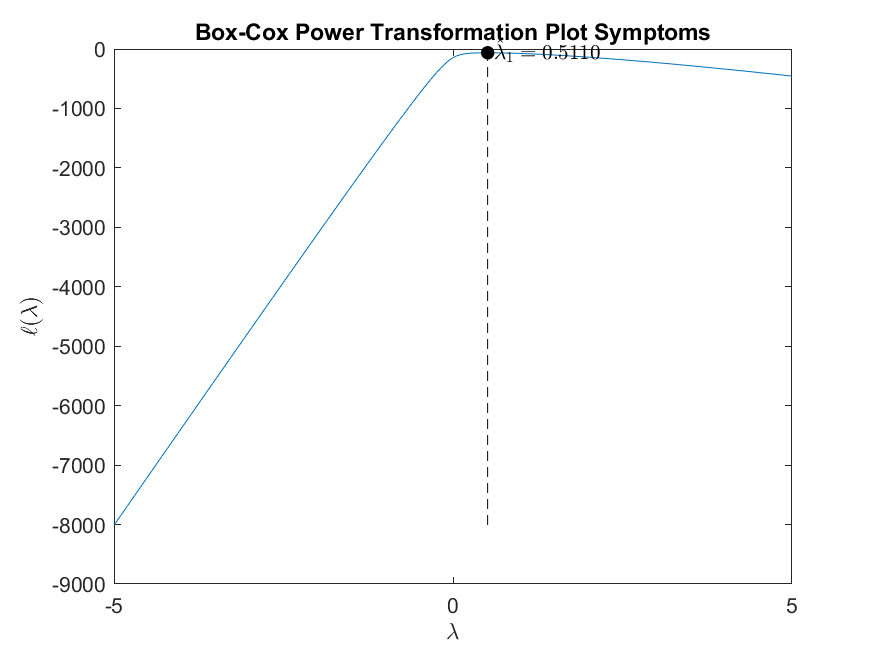
\includegraphics[scale=0.6]{./matlab/chapter-4/sol4.32.power.1.png}
    \end{figure}
\end{center}

\begin{center}
    \begin{figure}[H]
        \centering
        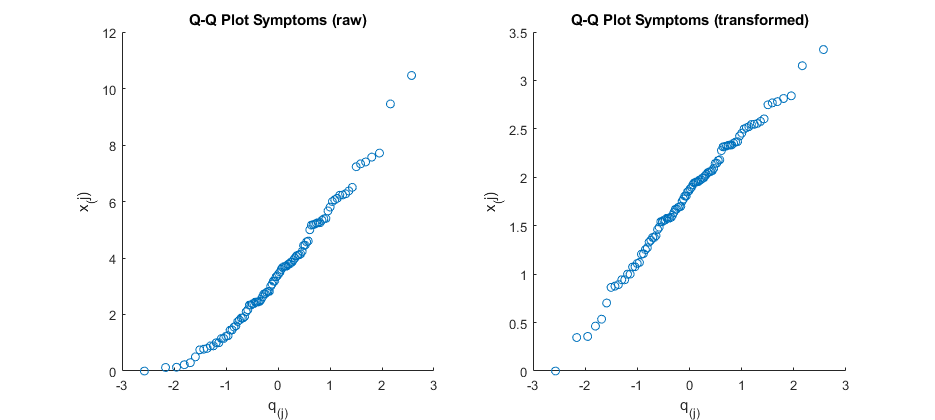
\includegraphics[scale=0.4]{./matlab/chapter-4/sol4.32.qq.1.png}
    \end{figure}
\end{center}

For activity ($x_{2}$), we're measuring patient activity on a continuous scale from 1 to 5, and have 97 valid observations. The Q-Q correlation on the raw data was 0.9455. The simulated 0.01, 0.05, and 0.10 level critical correlation coefficient test values for a sample size of 97 are, 0.9818, 0.9870, and 0.9892, respectively. Our Q-Q correlation value (0.9455) is smaller than all of these, so out data is not considered normally distributed at any of the 3 levels.

The Box-Cox power transformation is maximized at -0.4910, but I chose to round it to -0.50, so $x_{2}^{\prime} = 1/\sqrt{x_{2}}$. The Q-Q correlation coefficient on the transformed data was increased to 0.9630. This value is still smaller than the critical values at all three levels, but hey, it is an improvement. I'd say the problem with this variable is repeated values. We're measuring patient activity on a continous scale from 1 to 5. There are 16 of the 97 patiens (16.5\%) with an activity level of 1. These 16 values are creating a flat area in the Q-Q plot that cannot be fixed by any common transformation.

\begin{center}
    \begin{figure}[H]
        \centering
        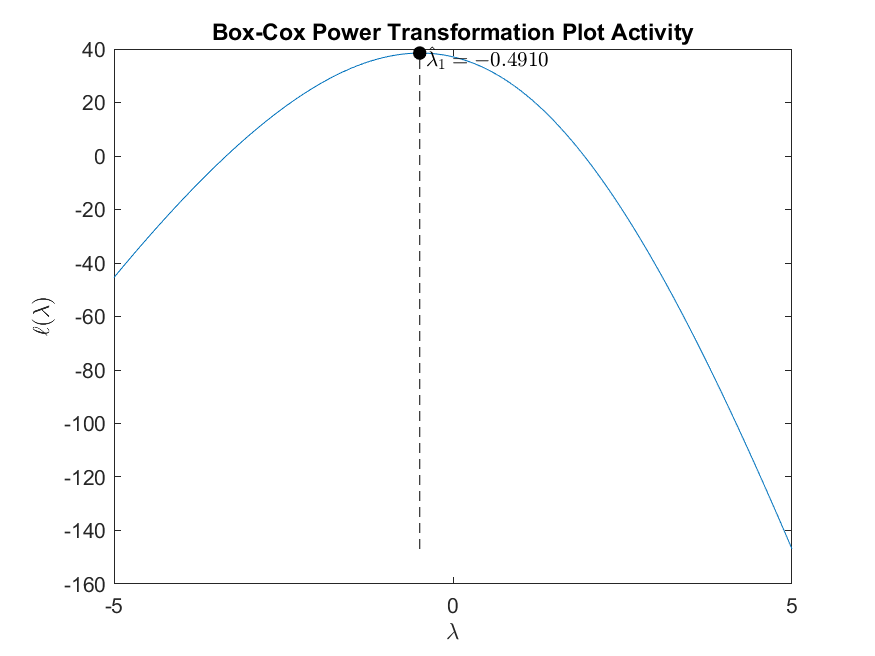
\includegraphics[scale=0.6]{./matlab/chapter-4/sol4.32.power.2.png}
    \end{figure}
\end{center}

\begin{center}
    \begin{figure}[H]
        \centering
        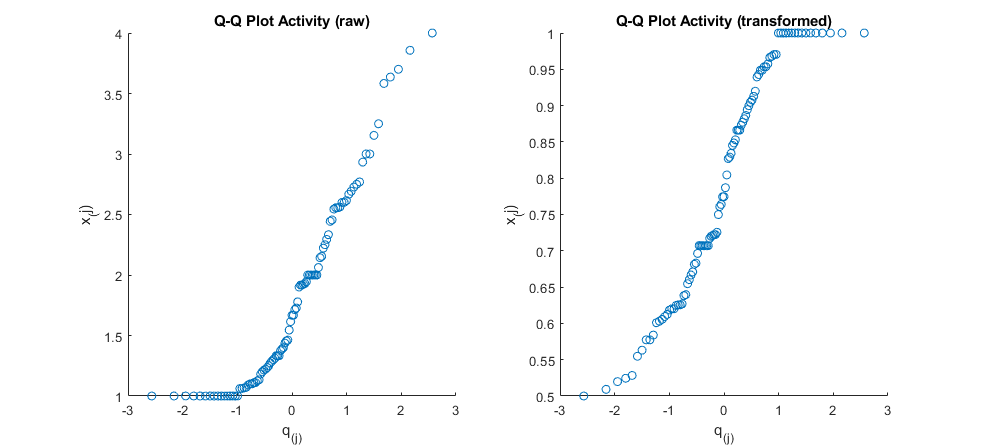
\includegraphics[scale=0.4]{./matlab/chapter-4/sol4.32.qq.2.png}
    \end{figure}
\end{center}

For sleep ($x_{3}$), we're measuring patient sleep on a continuous scale from 1 to 5, and have 94 valid observations. The simulated 0.01, 0.05, and 0.10 level critical correlation coefficient test values for a sample size of 94 are, 0.9812, 0.9867, and 0.9889, respectively. Our Q-Q correlation value of 0.9895 is larger than all of these, so out data is actually considered normally distributed at all 3 levels. Because of this I won't really bolther displaying the Box-Cox transformation results, but the power transformation of 0.7114 (close to 1) bumps the Q-Q correlation coefficient up slightly to 0.9893. The raw data Q-Q plot is below.

\begin{center}
    \begin{figure}[H]
        \centering
        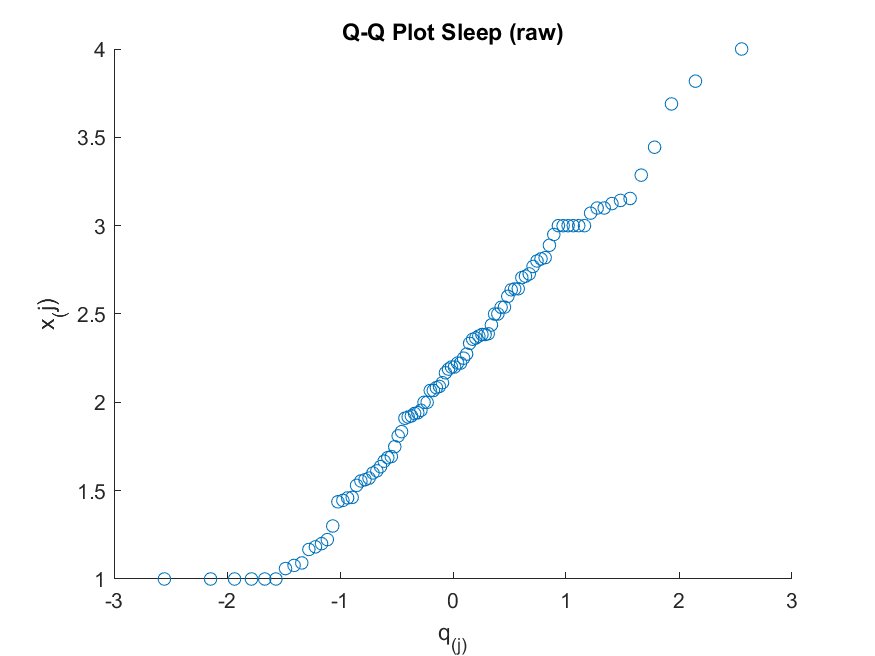
\includegraphics[scale=0.6]{./matlab/chapter-4/sol4.32.qq.3.png}
    \end{figure}
\end{center}

For eat ($x_{4}$), we're measuring amount of food consumed on a continuous scale from 1 to 3, and have 98 valid observations. The Q-Q correlation on the raw data was 0.9810. The simulated 0.01, 0.05, and 0.10 level critical correlation coefficient test values for a sample size of 98 are, 0.9819, 0.9871, and 0.9893, respectively. Our Q-Q correlation value (0.9810) is smaller than all of these, so out data is not considered normally distributed at any of the 3 levels.

The Box-Cox power transformation is maximized at 0.2305, but I chose to round it to 0.25, so $x_{4}^{\prime} = \sqrt[4]{x_{4}}$. The Q-Q correlation coefficient on the transformed data was increased slightly to 0.9834. This value is larger than the critical value at the 0.01-level (0.9819), but still smaller than the critical values at 0.05 and 0.01 levels. In this case our transformation has improved the normality of our data, if only slightly. I should also note that most of the data is tightly clustered, with the exception of observation 13, who has an eat value lower than the others with value 1.2826 and standardized residual of -2.8.

\begin{center}
    \begin{figure}[H]
        \centering
        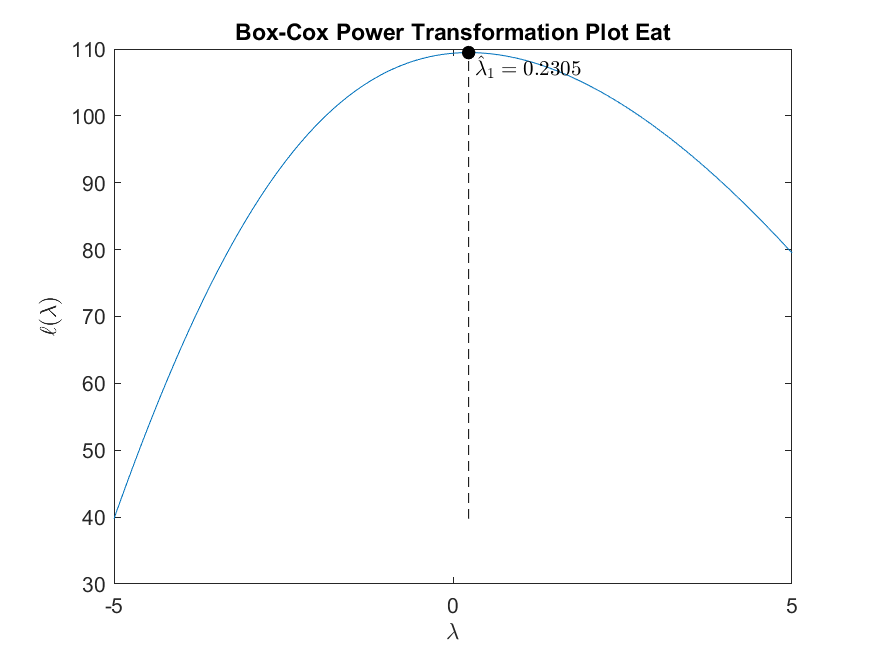
\includegraphics[scale=0.6]{./matlab/chapter-4/sol4.32.power.4.png}
    \end{figure}
\end{center}

\begin{center}
    \begin{figure}[H]
        \centering
        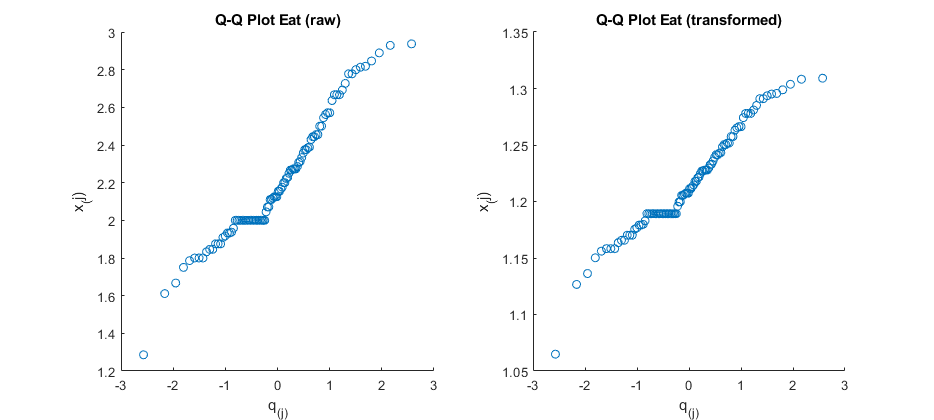
\includegraphics[scale=0.4]{./matlab/chapter-4/sol4.32.qq.4.png}
    \end{figure}
\end{center}

For appetite ($x_{5}$), we're measuring patient appetite on a continuous scale from 1 to 5, and have 98 valid observations. The simulated 0.01, 0.05, and 0.10 level critical correlation coefficient test values for a sample size of 94 are, 0.9819, 0.9871, and 0.9893, respectively. Our Q-Q correlation value of 0.9906 is larger than all of these, so out data is actually considered normally distributed at all 3 levels. Because of this I won't really bolther displaying the Box-Cox transformation results, but the power transformation of 0.6112 bumps the Q-Q correlation coefficient up slightly to 0.9924. The raw data Q-Q plot is below.

\begin{center}
    \begin{figure}[H]
        \centering
        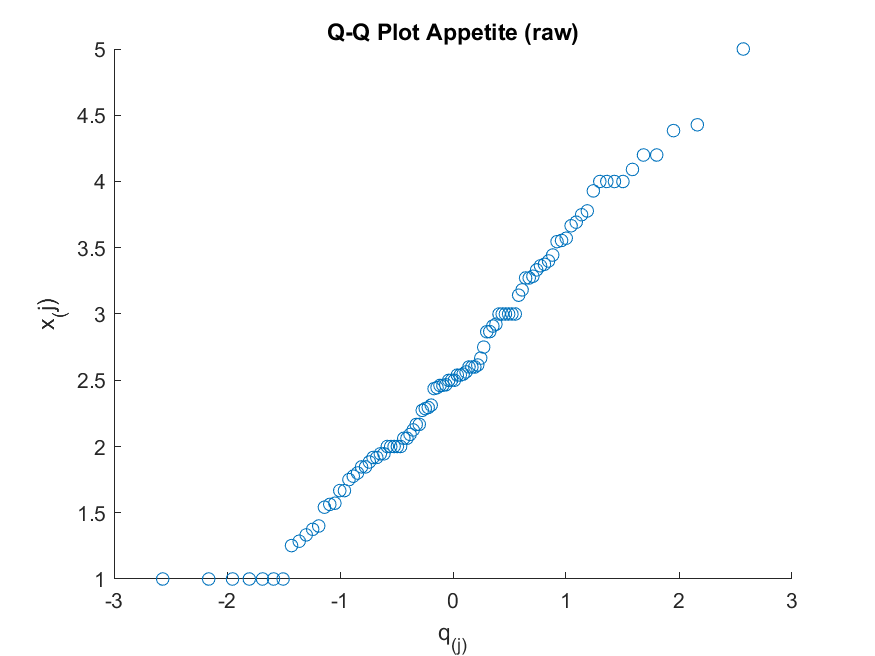
\includegraphics[scale=0.6]{./matlab/chapter-4/sol4.32.qq.5.png}
    \end{figure}
\end{center}

For skin reaction ($x_{6}$), we're measuring amount of skin reaction on a discrete scale from 0 to 3, and have 98 valid observations. The problem here is that the daata is discrete, so I would think a transformation might not be appropriate since this would be considered a factor varaible. I'll do the work anyway just to see what happens.

The Q-Q correlation on the raw data was 0.9278. The simulated 0.01, 0.05, and 0.10 level critical correlation coefficient test values for a sample size of 98 are, 0.9819, 0.9871, and 0.9893, respectively. Our Q-Q correlation value (0.9278) is smaller than all of these, so out data is not considered normally distributed at any of the 3 levels.

The Box-Cox power transformation is maximized at 0.2705, so $x_{6}^{\prime} = x_{6}^{0.2705}$. The Q-Q correlation coefficient on the transformed data was decreased to 0.8371. This value is worse than the one for the raw data and so still not larger than any of the 3 critical points. The Q-Q plot on the raw data is below. Just like for the activity variable we have lots of flat spots, so it's unlikely a common transformation will increase the Q-Q correlation value high enough to be larger than any of the critical points. It probably best to use the raw data for analysis or use it as a factor variable.

\begin{center}
    \begin{figure}[H]
        \centering
        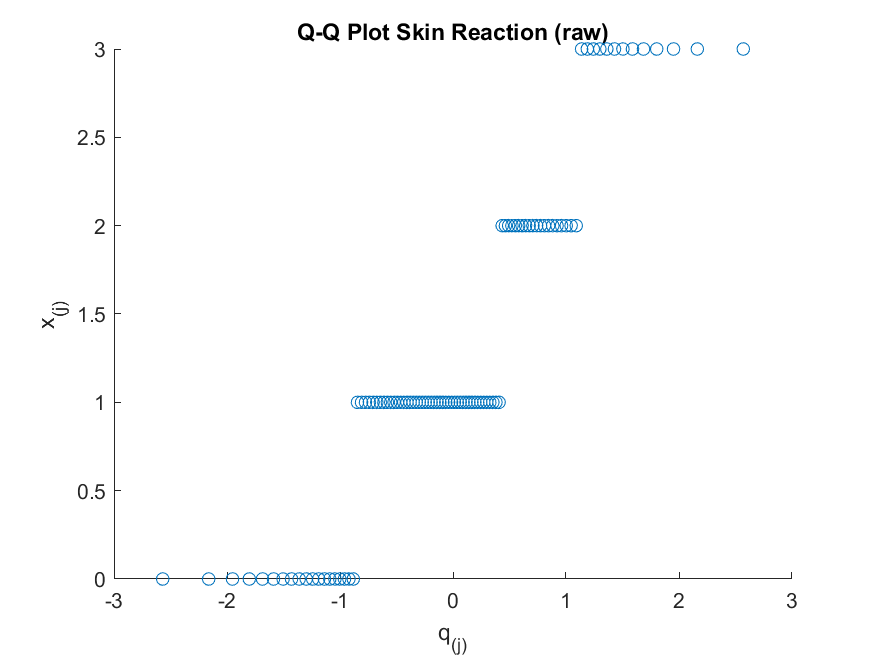
\includegraphics[scale=0.6]{./matlab/chapter-4/sol4.32.qq.6.png}
    \end{figure}
\end{center}